\chapter{Collision Data Samples}
\label{chap:data}
\section{Data Periods and Good Run List}
\label{EventSel:GRL}

\indent This analysis uses the data collected by the ATLAS experiment in 2015 and 2016 from the LHC proton-proton collisions at a centre-of-mass energy of $\sqrt{s}$=13 TeV. \\

\indent We select for data where all relevant subdetector parts are running without defects and the data quality is good.  This is done by requiring the data pass a good run list (GRL).  The good run list is compiled after checks has been performed on the data using combination of online monitoring of the detector hardware and checks that the kinematics of reconstructed physics objects agrees with expected distributions both online and offline.  \\

\indent The GRLs used for the 2015 dataset is {\tt \scriptsize data15\_13TeV.periodAllYear\_DetStatus-v79-repro20-02\_DQDefects-00-02-02\_PHYS\_StandardGRL\_All\_Good\_25ns.xml}.  The GRL\\
The GRL for the 2016 data is {\tt \scriptsize data16\_13TeV.periodAllYear\_DetStatus-v83-pro20-15\_DQDefects-00-02-04\_PHYS\_StandardGRL\_All\_Good\_25ns.xml}.

\indent The dataset after GRL selection has a total integrated luminosity of $\intlumi \pm 1.2$ $\ifb$.  The total integrated luminosity vs time for 2015 and 2016 can be seen in figure \ref{fig:data2015-2016}.\\

\begin{figure}[htb]
  \begin{center}
    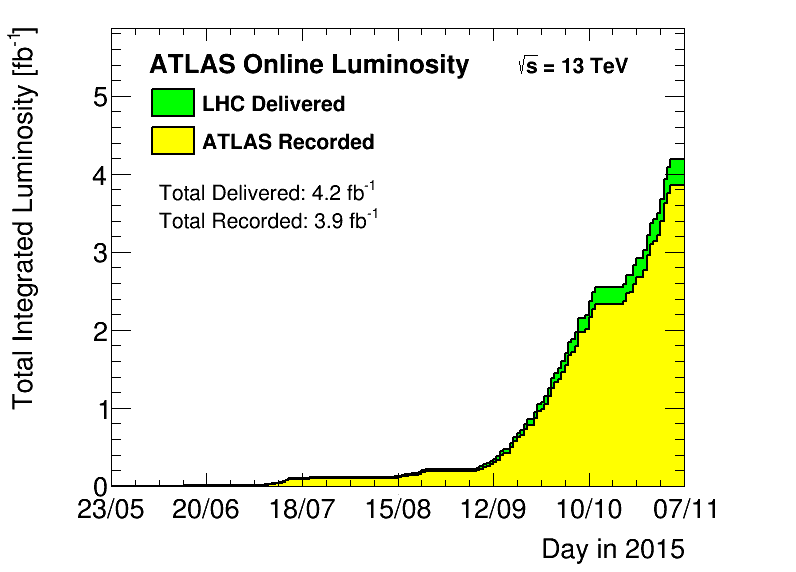
\includegraphics[width=0.45\textwidth]{figures/Data/IntLumi2015.png}\hspace{0.05\textwidth}
    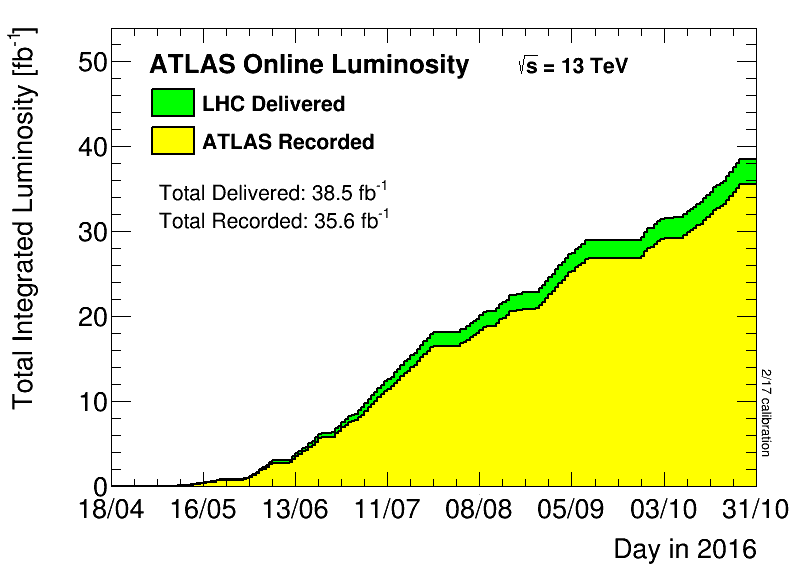
\includegraphics[width=0.45\textwidth]{figures/Data/IntLumi2016.png}\hspace{0.05\textwidth}
\end{center}
\caption{Distribution of the amount of data delivered by the LHC and recorded ATLAS vs time in 2015 and 2016  }
\label{fig:data2015-2016} 
\end{figure}

\indent Peak luminosity reached $1.38 \times 10^{34}$  cm$^{-2}$ sec$^{-1}$ in 2016.  Taking data at this rate means that there will be multiple proton proton interactions every bunch crossing.  This can be seen as the distribution of the mean number of interactions per bunch crossing weighted by luminosity shown in figure \ref{fig:nVtx}.  The average number of interactions per bunch crossing ($\braket{\mu}$) is 13.7 in 2015 and 23.2 in 2016. \\

\begin{figure}[htb]
  \begin{center}
    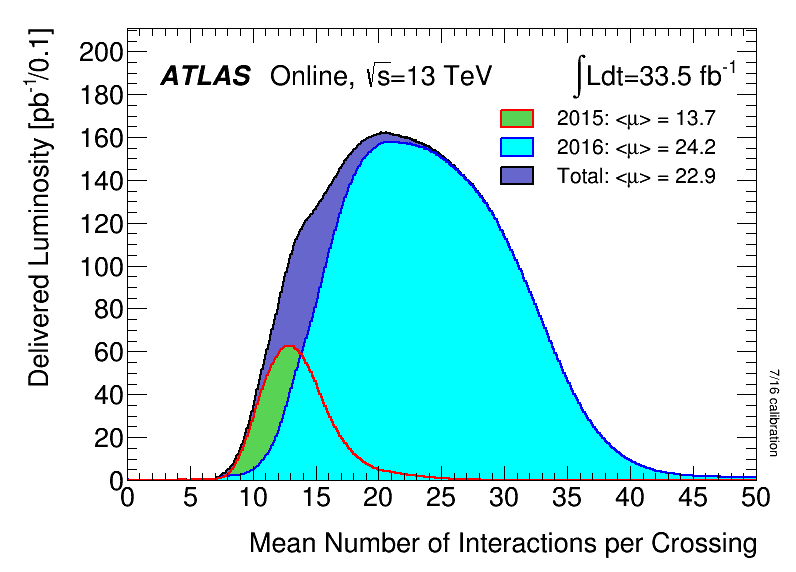
\includegraphics[width=0.55\textwidth]{figures/Data/mu_2015_2016_LHCC.png}\hspace{0.05\textwidth}
\end{center}
\caption{Distribution of the mean number of interactions per bunch crossing weighted by integrated luminosity in 2015 and 2016  }
\label{fig:nVtx} 
\end{figure}

\indent We use $\met$ only trigger for signal selection. Details on the ATLAS triggering system and the $\met$ trigger can be found in chapter \ref{chap:trigger}.  \\

\indent This analysis uses the lowest unprescaled $\met$ trigger with the best turn-on curve available for each data taking period.  This trigger is {\tt HLT\_xe70\_tc\_lcw} for all of 2015 data taking, \verb+HLT_xe90_mht_L1XE50+ for 2016 period A-D3, \verb+HLT_xe100_mht_L1XE50+ for 2016 period D4-F1, and \verb+HLT_xe110_mht_L1XE50+ for 2016 period F2 and onward.\\



\chapter{Event Preselection}
\label{sec:Selection_EventPreselection}

\indent We first require that the event pass a few {\it event cleaning}, and {\it jet cleaning} in addition to requirements on the Good Run List (GRL) selections. These selections ensure that the event does not have large amounts of calorimeter noise or non-collision backgrounds such as cosmic muons which may lead to fake jets or poor $\met$ reconstruction. These basic selections are applied to all control regions (CR), validation regions (VR), and signal regions (SR).  \\

\indent A brief description of each selection is given below: \\

\begin{description}
\item[Cut 1] Data events must be in accepted according to the Good Runs List (GRL) described in chapter \ref{EventSel:GRL}.  This ensures all relevant subdetector of ATLAS are operating normally during data taking. 
\item[Cut 2] Remove events with noise bursts and possible incomplete events due to the TTC reset procedure from the data. Data events must have larError $== 0$, tileError $== 0$, SCT error $==0$, and coreFlags $\&0x4000 == 0$.
\item[Cut 4] Require that at least one reconstructed primary vertex must exist.
\item[Cut 5] Events must not contain any {\tt BadLoose} jets with $\pT > 20 \gev$ (at any \eta\ range). {\tt BadLoose} jets are defined in jet quality selection in section \ref{sec:jet:quality}.  Bad quality jets corresponds with calorimeter noise or non-collision backgrounds both of which leads to poor $\met$ reconstruction.
\item[Cut 6] The event must not contain any cosmic muons.  Cosmic muons are identified as muons with large impact parameters  ($|z_0| > 1$ mm and $|d_0| > 0.2$ mm).  Only baseline muons after overlap removal are considered.
\item[Cut 7] The event must not contain any bad muons.  Event must not contain any muon reconstructed from high hit multiplicities in the muon spectrometer due to high jets punching through the calorimeter and depositing energy into the muon system, or from poorly reconstructed inner detector tracks from jets incorrectly matched to muon spectrometer segments. Such {\it fake} muons make result in misreconstructed $\met$ so the whole event is rejected.
\end{description}

\indent On top of these basic selections, a set of specific set of {\it pre-selection} is applied to each control, validation and signal region depending on the number of leptons required in the respective region.  \\

\indent Any 0 lepton region require the selections given in table \ref{tab:0Lcommon}. \\

\begin{table}[htbp]
  \caption{ 0  lepton pre-selection criteria common to all 0 lepton signal and validation regions.}
  \begin{center}
    \begin{tabular}{l|c} \hline\hline
      \multicolumn{2}{c}{GRL, Event Cleaning and Jet Cleaning} \\
      Trigger & Data 2015: \verb+HLT_xe70_mht_L1XE50+ \\ %\hline
              & Data 2016 (period A-D3): \verb+HLT_xe90_mht_L1XE50+ \\  
              & Data 2016 (period D4-F1): \verb+HLT_xe100_mht_L1XE50+  \\ 
              & Data 2016 (period F2 and onward): \verb+HLT_xe110_mht_L1XE50+  \\ %\hline
              & \\ [-2.5ex] \hline
      $\met$ & $> 250\GeV$ \\ %\hline
              & \\ [-2.5ex] \hline
      $N_{\rm{baseline lep}}$ & 0 \\ \hline
      \antikt\ $R=0.4$ signal jets & $\ge 4,~\pt>80,80,40,40 \gev$ \\ \hline
      $b$-tagged signal jets & $\ge1$ \\ \hline
      % $\dphijettwomet$ & $> \pi/5$ \\ 
      $\dphijettwomet$ & $> 0.4$ \\ 
              & \\ [-2.5ex] \hline
      $\mettrk$  & $> 30 \gev$ \\ \hline 
      % & \\ [-2.5ex]
      $\dphimettrk$ & $<\pi/3$ \\ \hline
      % & \\ [-2.5ex] \hline
      % $\tau$ veto & yes \\ \hline
      % $\mtbmetmindphi$ & $> 175 \gev$ \\ \hline \hline
    \end{tabular}
  \end{center}
  \label{tab:0Lcommon}
\end{table}

\indent All 0 lepton regions trigger on $\met$ using the lowest unprescaled $\met$ trigger for that data period.  Details on the $\met$ trigger can be found in chapter \ref{chap:trigger}.  An offline selection of $\met > 250 \gev$ is required to ensure that all accepted events are on the triggering efficiency plateau.  Trigger efficiency vs offline $\met$ can be seen in figure \ref{fig:trigTurnON}.  \\

\indent The event must contain exactly zero baseline leptons since this is a 0 lepton region. \\

\indent We then require at least four signal jets with a minimum pt of $(80,80,40,40) \gev$ in the event.  At least one signal jet must be b-tagged with the 77 percent working point.  This jet energy and multiplicity requirement is loose and will be superseded by other selections in each SR, VR and CR.  \\

\indent If the $\met$ is too close to either of two most energetic jets in the event then the event is rejected. The $\met$ could be resulting from an misreconstructed energetic jet.  \\

\indent Misreconstructed jets is primary reason that QCD multijets background which produces little intrinsic $\met$ are accepted by the signal selection.  For example an extremely energetic jet may punch through the calorimeter and be reconstructed with less $E_T$.  This lost $E_T$ maybe reconstructed as $\met$.  The $\dphijettwomet > 0.4$ provide strong discrimination power against the QCD multijet background. \\

\indent The selections on the presence of $\mettrk$ and loose agreement in direction between $\met$ and $\mettrk$ are required to also discriminate against $\met$ resulting from misreconstructed jets. \\

\indent Details on all object definitions are given in chapter \ref{chap:objects}.

\indent Any 1 lepton region require the selections given in table \ref{tab:1Lcommon}. 

\begin{table}[htbp]
  \caption{ 1 lepton pre-selection criteria common to all 1 lepton signal and validation regions.}
  \begin{center}
    \begin{tabular}{l|c} \hline\hline
      \multicolumn{2}{c}{GRL, Event Cleaning and Jet Cleaning} \\
      Trigger & Data 2015: \verb+HLT_xe70_mht_L1XE50+ \\ %\hline
              & Data 2016 (period A-D3): \verb+HLT_xe90_mht_L1XE50+ \\  
              & Data 2016 (period D4-F1): \verb+HLT_xe100_mht_L1XE50+  \\ 
              & Data 2016 (period F2 and onward): \verb+HLT_xe110_mht_L1XE50+  \\ %\hline
              & \\ [-2.5ex] \hline
      $\met$ & $> 250\GeV$ \\ %\hline
              & \\ [-2.5ex] \hline
      $N_{\rm{signal lep}}$ & 1 \\ \hline
    $N_{jets}$ & $\ge 4$ \\ \hline
      $b$-tagged signal jets & $\ge1$ \\ \hline
      $\dphijettwomet$ & $> 0.4$ \\
              & \\ [-2.5ex] \hline
    \end{tabular}
  \end{center}
  \label{tab:1Lcommon}
\end{table}

\indent The 1 lepton preselection is similar to the 0 lepton preselection except for several important requirements. First, the 1 lepton selections are made on signal leptons instead of baseline leptons in 0 lepton regions.  The 1 lepton regions require high quality leptons because we use their momenta measurements instead of only vetoing on leptons.  \\

\indent Next both signal leptons and signal $R=0.4$ $\antikt$ jets are counted as {\it jets} in 1 lepton regions.  This is because 1 lepton regions are all control and validation regions that are meant to model the background in the signal region.  The biggest background contributions in the signal region are backgrounds that decay through the hadronic tau channel.  We can use the electron and muons decay channels to model the tau decay channel because of lepton universality.  In this case, we use the measured electron and muon four momenta to model the four momenta of the hadronic tau jet that we expect in the signal region.  Leptons are never counted as b-tagged jets.  \\

\indent The $\mettrk > 30 \gev$ and $\dphimettrk < \pi/3$ requirements are removed because the QCD multijet contribution to the 1 lepton region is negligible.  $\dphijettwomet > 0.4$ selection is kept because it does affect the phase space of accepted events for some backgrounds such as ttbar.  Keeping the cut provides a closer modeling of those background in the SR. \\